\documentclass[tikz, border=4pt]{standalone}
\usepackage{tikz}
\usepackage{circuitikz}
\begin{document}
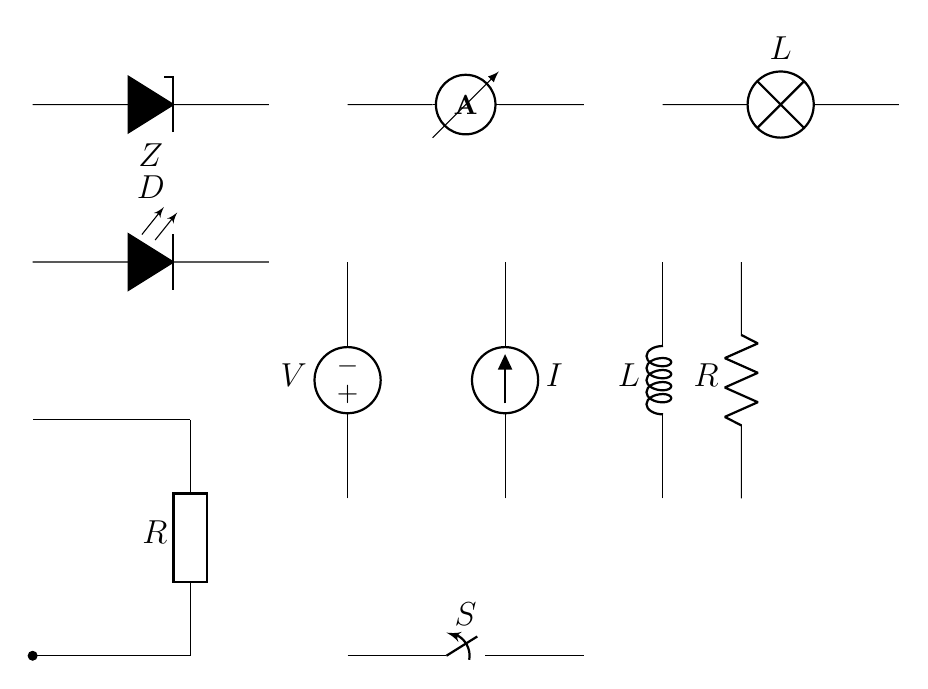
\begin{tikzpicture}[x=1cm, y=1cm]
  \begin{scope}[shift={(0,0)}, font=\large]
    \draw (0,0) to[short, *-] (2,0);
    \draw (2,0) to[european resistor, l=$R$] (2,3);
    \draw (2,3) -- (0,3);
    \draw (4,0) to[ospst, l=$S$] (7,0);
    \draw (4,2) to[american voltage source, l=$V$] (4,5);
    \draw (6,2) to[american current source, l_=$I$] (6,5);
    \draw (8,2) to[cute inductor, l=$L$] (8,5);
    \draw (9,2) to[american resistor, l=$R$] (9,5);
    \draw (0,5) to[leD*, l=$D$] (3,5);
    \draw (0,7) to[zD*, l_=$Z$] (3,7);
    \draw (4,7) to[ammeter] (7,7);
    \draw (8,7) to[lamp, l=$L$] (11,7);
  \end{scope}
\end{tikzpicture}
\end{document}
